% ============================================================================================================
\chapter{Les stratégies S1 à S5 réévaluées}\label{ch:strategies}
% ============================================================================================================

Les cinq stratégies sont recalculées avec exactement les mêmes mesures qu'en v0.7 (tableau~\ref{tab:strat_def}), dans
trois configurations explicites :
\begin{itemize}
\item \textbf{centrale} : tous les paramètres à leur valeur centrale ;
\item \textbf{réactions faibles, transmission lente} : élasticités d'offre de travail basses, épargne de précaution
faible, pas de rigidité salariale asymétrique, transfert de bénéfices faible, pas de canal de trésorerie ni de
délocalisation, aucune incidence salariale de l'IS et des impôts de production, cotisations entièrement transmises
aux salaires, R\&D peu additionnelle, θ = 0,5, ρ = 0,1 ;
\item \textbf{réactions fortes, transmission rapide} : les valeurs hautes correspondantes, θ = 1,0, ρ = 0,3.
\end{itemize}
Ces deux configurations ne sont pas « favorable » et « défavorable » par construction : selon la stratégie, des
réactions plus fortes peuvent améliorer l'activité et dégrader la dette, ou l'inverse. Pour chaque stratégie, la
configuration la plus favorable et la plus défavorable sur chaque indicateur sont lues a posteriori (crochets du
tableau~\ref{tab:strat_configs}).

\begin{table}[htbp]\centering\scriptsize
\caption{Mesures des stratégies (écart à la situation actuelle ; identiques à la v0.7).}\label{tab:strat_def}
\tabfit{../../../phase3/rapport/tables/strategies_principal.tex}
\end{table}

\section{Effets par horizon}

{\small\setlength{\tabcolsep}{4pt}\begin{longtable}{llrrrrr}\caption{Stratégies S1 à S5 (définitions de la v0.7) avec le modèle v0.8 : écarts à la référence, configuration centrale.}\label{tab:strat_horizons}\\ \toprule Stratégie & Indicateur & 2027 & 2030 & 2035 & 2040 & 2047\\ \midrule\endfirsthead \toprule Stratégie & Indicateur & 2027 & 2030 & 2035 & 2040 & 2047\\ \midrule\endhead
S1 Protection & PIB (\%) & $+0{,}00$ & $+1{,}77$ & $+0{,}69$ & $+0{,}10$ & $-0{,}32$\\
 & PIB potentiel (\%) & $+0{,}00$ & $+0{,}20$ & $+0{,}00$ & $-0{,}34$ & $-0{,}74$\\
 & Emploi (milliers) & $+0$ & $+643$ & $+600$ & $+400$ & $+333$\\
 & Chômage (pt) & $+0{,}00$ & $-1{,}35$ & $-1{,}21$ & $-0{,}62$ & $-0{,}43$\\
 & Coût salarial (\%) & $+0{,}00$ & $+0{,}84$ & $+4{,}17$ & $+5{,}90$ & $+6{,}72$\\
 & RDB nominal (\%) & $+0{,}00$ & $+6{,}09$ & $+9{,}02$ & $+10{,}37$ & $+11{,}10$\\
 & Recettes (pt) & $+0{,}00$ & $+0{,}32$ & $+0{,}45$ & $+0{,}45$ & $+0{,}39$\\
 & Dépenses (pt) & $+0{,}00$ & $+0{,}98$ & $+1{,}17$ & $+1{,}57$ & $+2{,}14$\\
 & Solde (pt) & $+0{,}00$ & $-0{,}67$ & $-0{,}72$ & $-1{,}12$ & $-1{,}74$\\
 & Dette (pt) & $+0{,}0$ & $-0{,}6$ & $-0{,}7$ & $+2{,}2$ & $+9{,}7$\\
 & Coût salarial réel (\%) & $+0{,}00$ & $+0{,}16$ & $+1{,}06$ & $+1{,}77$ & $+2{,}30$\\
 & Part de l'industrie (pt) & $+0{,}00$ & $-0{,}09$ & $-0{,}14$ & $-0{,}17$ & $-0{,}13$\\
 & RDB réel des ménages (\%, M16) & $+0{,}00$ & $+6{,}06$ & $+6{,}62$ & $+6{,}93$ & $+7{,}28$\\
 & Niveau de vie médian réel (\%) & $+0{,}00$ & $+9{,}32$ & $+9{,}64$ & $+9{,}94$ & $+10{,}26$\\
 & Pauvreté, seuil fixe (pt) & $+0{,}00$ & $-4{,}28$ & $-4{,}32$ & $-4{,}15$ & $-4{,}13$\\
 & Gini (×100) & $-0{,}08$ & $-2{,}24$ & $-2{,}12$ & $-1{,}94$ & $-1{,}84$\\
\addlinespace
S2 Emploi & PIB (\%) & $+0{,}00$ & $+1{,}34$ & $+1{,}30$ & $+1{,}50$ & $+1{,}81$\\
 & PIB potentiel (\%) & $+0{,}00$ & $+0{,}56$ & $+1{,}27$ & $+1{,}76$ & $+2{,}25$\\
 & Emploi (milliers) & $+0$ & $+374$ & $+360$ & $+273$ & $+262$\\
 & Chômage (pt) & $+0{,}00$ & $-0{,}64$ & $-0{,}59$ & $-0{,}34$ & $-0{,}31$\\
 & Coût salarial (\%) & $+0{,}00$ & $-1{,}49$ & $-0{,}41$ & $+0{,}08$ & $+0{,}18$\\
 & RDB nominal (\%) & $+0{,}00$ & $+0{,}96$ & $+1{,}76$ & $+1{,}99$ & $+1{,}98$\\
 & Recettes (pt) & $+0{,}00$ & $+0{,}18$ & $+0{,}20$ & $+0{,}18$ & $+0{,}17$\\
 & Dépenses (pt) & $+0{,}00$ & $+0{,}91$ & $+1{,}19$ & $+1{,}81$ & $+3{,}56$\\
 & Solde (pt) & $+0{,}00$ & $-0{,}73$ & $-1{,}00$ & $-1{,}63$ & $-3{,}39$\\
 & Dette (pt) & $+0{,}0$ & $+2{,}2$ & $+5{,}1$ & $+10{,}7$ & $+25{,}6$\\
 & Coût salarial réel (\%) & $+0{,}00$ & $-0{,}97$ & $-0{,}43$ & $+0{,}02$ & $+0{,}27$\\
 & Part de l'industrie (pt) & $+0{,}00$ & $-0{,}02$ & $-0{,}03$ & $-0{,}02$ & $+0{,}03$\\
 & RDB réel des ménages (\%, M16) & $+0{,}00$ & $+0{,}76$ & $+1{,}13$ & $+1{,}36$ & $+1{,}51$\\
 & Niveau de vie médian réel (\%) & $+0{,}00$ & $+3{,}09$ & $+3{,}40$ & $+3{,}61$ & $+3{,}76$\\
 & Pauvreté, seuil fixe (pt) & $+0{,}00$ & $-1{,}49$ & $-1{,}56$ & $-1{,}51$ & $-1{,}52$\\
 & Gini (×100) & $-0{,}08$ & $-1{,}06$ & $-1{,}01$ & $-0{,}92$ & $-0{,}88$\\
\addlinespace
S3 Productivité & PIB (\%) & $+0{,}00$ & $+1{,}94$ & $+2{,}30$ & $+3{,}15$ & $+4{,}33$\\
 & PIB potentiel (\%) & $+0{,}00$ & $+1{,}01$ & $+2{,}58$ & $+4{,}11$ & $+5{,}59$\\
 & Emploi (milliers) & $+0$ & $+535$ & $+622$ & $+714$ & $+971$\\
 & Chômage (pt) & $+0{,}00$ & $-0{,}51$ & $+0{,}07$ & $+0{,}80$ & $+0{,}93$\\
 & Coût salarial (\%) & $+0{,}00$ & $+0{,}27$ & $+1{,}07$ & $+0{,}49$ & $-1{,}13$\\
 & RDB nominal (\%) & $+0{,}00$ & $+3{,}39$ & $+4{,}35$ & $+3{,}82$ & $+2{,}74$\\
 & Recettes (pt) & $+0{,}00$ & $-0{,}66$ & $-0{,}69$ & $-0{,}76$ & $-0{,}78$\\
 & Dépenses (pt) & $+0{,}00$ & $+0{,}99$ & $+1{,}48$ & $+2{,}37$ & $+5{,}83$\\
 & Solde (pt) & $+0{,}00$ & $-1{,}66$ & $-2{,}17$ & $-3{,}14$ & $-6{,}60$\\
 & Dette (pt) & $+0{,}0$ & $+2{,}7$ & $+10{,}0$ & $+22{,}3$ & $+53{,}3$\\
 & Coût salarial réel (\%) & $+0{,}00$ & $+0{,}10$ & $+0{,}52$ & $+0{,}59$ & $+0{,}09$\\
 & Part de l'industrie (pt) & $+0{,}00$ & $-0{,}09$ & $-0{,}13$ & $-0{,}12$ & $-0{,}09$\\
 & RDB réel des ménages (\%, M16) & $+0{,}00$ & $+3{,}65$ & $+4{,}31$ & $+4{,}41$ & $+4{,}54$\\
 & Niveau de vie médian réel (\%) & $+0{,}00$ & $+6{,}99$ & $+7{,}32$ & $+6{,}99$ & $+6{,}80$\\
 & Pauvreté, seuil fixe (pt) & $+0{,}00$ & $-2{,}53$ & $-2{,}34$ & $-2{,}12$ & $-1{,}98$\\
 & Gini (×100) & $-0{,}08$ & $-1{,}35$ & $-1{,}04$ & $-0{,}76$ & $-0{,}57$\\
\addlinespace
S4 Redressement & PIB (\%) & $+0{,}00$ & $-0{,}40$ & $-0{,}53$ & $-0{,}55$ & $-0{,}49$\\
 & PIB potentiel (\%) & $+0{,}00$ & $-0{,}05$ & $-0{,}45$ & $-0{,}68$ & $-0{,}69$\\
 & Emploi (milliers) & $+0$ & $-77$ & $-68$ & $+13$ & $+62$\\
 & Chômage (pt) & $+0{,}00$ & $+0{,}23$ & $+0{,}20$ & $-0{,}04$ & $-0{,}18$\\
 & Coût salarial (\%) & $+0{,}00$ & $-0{,}12$ & $-0{,}82$ & $-1{,}21$ & $-1{,}34$\\
 & RDB nominal (\%) & $+0{,}00$ & $-1{,}20$ & $-1{,}99$ & $-2{,}01$ & $-1{,}76$\\
 & Recettes (pt) & $+0{,}00$ & $+1{,}10$ & $+1{,}08$ & $+1{,}10$ & $+1{,}12$\\
 & Dépenses (pt) & $+0{,}00$ & $-0{,}80$ & $-1{,}56$ & $-2{,}64$ & $-5{,}55$\\
 & Solde (pt) & $+0{,}00$ & $+1{,}90$ & $+2{,}64$ & $+3{,}75$ & $+6{,}68$\\
 & Dette (pt) & $+0{,}0$ & $-4{,}8$ & $-14{,}7$ & $-28{,}5$ & $-59{,}3$\\
 & Coût salarial réel (\%) & $+0{,}00$ & $-0{,}45$ & $-0{,}80$ & $-1{,}10$ & $-1{,}24$\\
 & Part de l'industrie (pt) & $+0{,}00$ & $+0{,}02$ & $+0{,}07$ & $+0{,}11$ & $+0{,}14$\\
 & RDB réel des ménages (\%, M16) & $+0{,}00$ & $-2{,}11$ & $-2{,}37$ & $-2{,}47$ & $-2{,}49$\\
 & Niveau de vie médian réel (\%) & $+0{,}00$ & $-1{,}52$ & $-1{,}73$ & $-1{,}81$ & $-1{,}85$\\
 & Pauvreté, seuil fixe (pt) & $+0{,}00$ & $+1{,}25$ & $+1{,}35$ & $+1{,}38$ & $+1{,}33$\\
 & Gini (×100) & $-0{,}08$ & $-0{,}07$ & $-0{,}10$ & $-0{,}11$ & $-0{,}15$\\
\addlinespace
S5 Global & PIB (\%) & $+0{,}00$ & $+0{,}36$ & $+0{,}52$ & $+0{,}68$ & $+0{,}86$\\
 & PIB potentiel (\%) & $+0{,}00$ & $+0{,}32$ & $+0{,}69$ & $+0{,}95$ & $+1{,}22$\\
 & Emploi (milliers) & $+0$ & $+79$ & $+122$ & $+139$ & $+169$\\
 & Chômage (pt) & $+0{,}00$ & $+0{,}10$ & $-0{,}02$ & $-0{,}07$ & $-0{,}16$\\
 & Coût salarial (\%) & $+0{,}00$ & $-1{,}94$ & $-2{,}36$ & $-2{,}70$ & $-3{,}02$\\
 & RDB nominal (\%) & $+0{,}00$ & $-0{,}12$ & $-0{,}51$ & $-0{,}83$ & $-1{,}09$\\
 & Recettes (pt) & $+0{,}00$ & $+0{,}69$ & $+0{,}71$ & $+0{,}72$ & $+0{,}71$\\
 & Dépenses (pt) & $+0{,}00$ & $+0{,}69$ & $+0{,}74$ & $+0{,}87$ & $+1{,}20$\\
 & Solde (pt) & $+0{,}00$ & $-0{,}00$ & $-0{,}03$ & $-0{,}15$ & $-0{,}49$\\
 & Dette (pt) & $+0{,}0$ & $+1{,}6$ & $+2{,}0$ & $+2{,}8$ & $+5{,}0$\\
 & Coût salarial réel (\%) & $+0{,}00$ & $-1{,}12$ & $-1{,}22$ & $-1{,}32$ & $-1{,}46$\\
 & Part de l'industrie (pt) & $+0{,}00$ & $+0{,}06$ & $+0{,}11$ & $+0{,}19$ & $+0{,}34$\\
 & RDB réel des ménages (\%, M16) & $+0{,}00$ & $-0{,}08$ & $-0{,}13$ & $-0{,}20$ & $-0{,}27$\\
 & Niveau de vie médian réel (\%) & $+0{,}00$ & $+1{,}97$ & $+1{,}96$ & $+1{,}93$ & $+1{,}85$\\
 & Pauvreté, seuil fixe (pt) & $+0{,}00$ & $-0{,}90$ & $-0{,}87$ & $-0{,}86$ & $-0{,}88$\\
 & Gini (×100) & $-0{,}08$ & $-0{,}86$ & $-0{,}87$ & $-0{,}89$ & $-0{,}92$\\\bottomrule\end{longtable}}

L'année 2027 précède la mise en œuvre (premier budget de la législature en 2028) : les écarts y sont nuls. Les
résultats sont relativement robustes jusqu'en 2030-2035 (les configurations encadrent la valeur centrale de quelques
dixièmes de point de PIB et de quelques points de dette) ; au-delà de 2040, l'incertitude devient dominante pour les
stratégies d'offre.

\begin{figure}[htbp]\centering
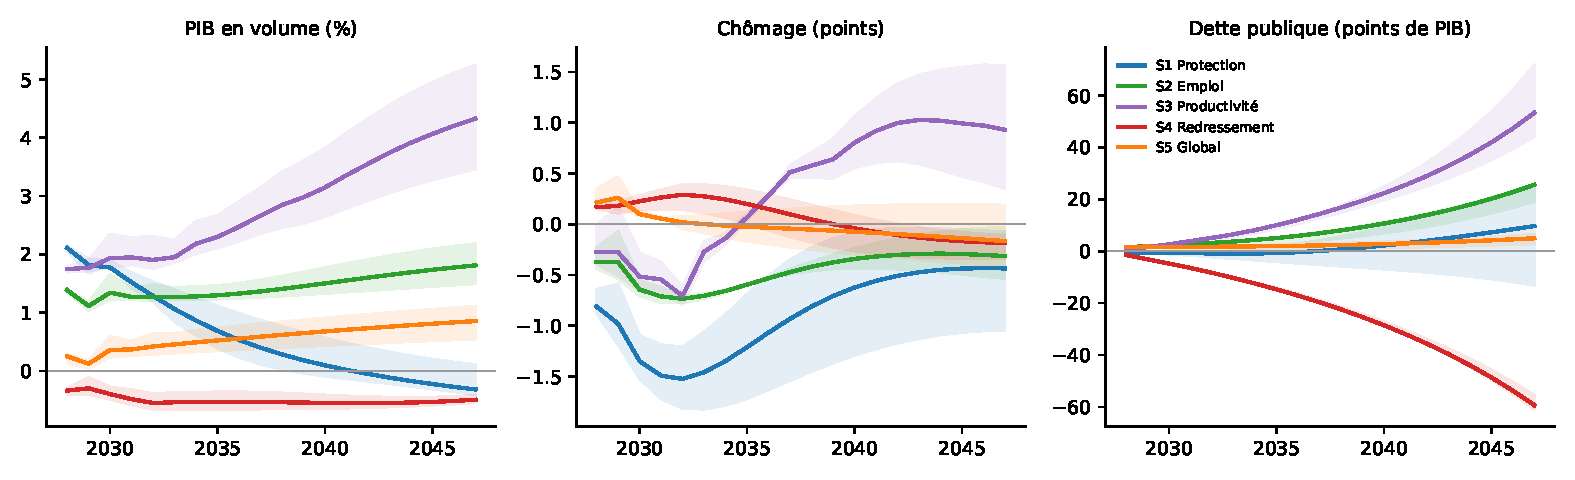
\includegraphics[width=\linewidth]{strategies_v08.pdf}
\caption{Stratégies S1 à S5 en v0.8 : configuration centrale (trait) et intervalle entre les configurations « réactions
faibles » et « réactions fortes » (bande).}\label{fig:strat_v08}
\end{figure}

\begin{table}[htbp]\centering\scriptsize
\caption{Valeur centrale et intervalle [min ; max] sur les trois configurations.}\label{tab:strat_configs}
\tabfit{../tables/strategies_configs.tex}
\end{table}

Les configurations ne font pas varier la prime de risque sur les taux français, dont l'effet sur la dette de long terme
est du même ordre que celui des comportements (chapitre~\ref{ch:sensibilite}) : avec une prime nulle ou haute (0 ou
0,05 point de taux par point de dette au lieu de 0,03), la dette de 2047 va de $+37$ à $+69$ points pour S3 et de $-44$ à
$-72$ points pour S4. Les horizons 2027-2035 sont peu touchés par cette hypothèse.

\section{Ce qui change par rapport à la v0.7}

\begin{table}[htbp]\centering\scriptsize
\caption{Effets des programmes en v0.7 et v0.8 (configuration centrale).}\label{tab:v07v08}
\tabfit{../tables/strategies_v07_v08.tex}
\end{table}

\begin{table}[htbp]\centering\scriptsize
\caption{Décomposition de l'écart v0.7 → v0.8 en 2047, configuration centrale : (a) correction du défaut de code, recalage de la référence, offre de travail en 18 cas types ; (b) fermeture estimée (θ, ρ, sans termes en différence) ; (c) incidence des prélèvements sur les entreprises.}\label{tab:decomp}
\tabfit{../tables/decomposition.tex}
\end{table}



\paragraph{La fermeture estimée explique l'essentiel des écarts.} Pour S2, S3 et S5, la colonne (b) domine : $+17$,
$+31$ et $+7$ points de dette en 2047. En v0.7, la demande anticipait 1,5 fois la hausse du potentiel (θ = 1,5) : la
production dépassait durablement son potentiel après une réforme d'offre, ce qui gonflait les recettes. Avec θ estimé
(0,75, plage 0,5-1,0), la production rejoint le potentiel accru sans le dépasser ; les recettes suivent, mais moins.
Le même mécanisme explique la révision des mesures d'offre prises isolément : le relèvement de l'âge légal à 65 ans
réduisait la dette de 8,5 points en 2047 en v0.7, de 1,9 point en v0.8 ; la durée du travail à 37 heures, de 18 points
en v0.7, de 1,4 point en v0.8. Leurs effets sur le PIB changent peu (1,2 et 1,7 \% en 2047).

\paragraph{La correction du défaut de code et le recalage} (colonne a) dégradent la dette de S1 de 6 points et celle de
S2, S3 et S5 de 3 à 6 points. Ces stratégies contiennent toutes une hausse de la prime d'activité, dont l'effet sur la
dette est révisé de $+2{,}9$ points par cette seule colonne (offre de travail en 18 cas types, recalage de la
référence) ; on ne peut pas séparer davantage ces deux causes sans simulations supplémentaires.

\paragraph{L'incidence des prélèvements sur les entreprises} (colonne c) dégrade la dette de S5 de 5,6 points et d'une
baisse de 20\md{} de cotisations de 4,1 points : en v0.7, la baisse de cotisations était entièrement transmise aux
salaires à long terme, ce qui soutenait le revenu des ménages et les recettes ; avec une transmission de moitié, une
partie va aux profits, moins taxés.

\begin{resultat}[Conclusions de la v0.7 invalidées]
\begin{itemize}
\item « S5 réduit la dette de 10 points en 2047 de façon robuste » : en v0.8, S5 l'\emph{augmente} de 5 points (3 à 6
selon la configuration ; $-2$ à $+4$ sans le module européen, selon l'incidence).
\item « S2 est neutre pour la dette » ($-0{,}8$ point) : en v0.8, $+26$ points (19 à 26).
\item « Les réformes d'offre (âge légal, durée du travail) réduisent fortement la dette » : leurs gains budgétaires
reposaient sur la fermeture de la v0.7 ; ils sont faibles en v0.8.
\item Les compositions optimisées en v0.7 pour S1, S2 et S3 ne respectent plus leur contrainte de dette quand elles sont
évaluées avec la v0.8 (chapitre~\ref{ch:optimisation}).
\end{itemize}
Restent valables : l'ordre des stratégies sur le PIB (S3 > S2 > S5 > S1 > S4) et sur la dette (S4 seule la réduit
nettement) ; la forte réduction de la pauvreté par S1 ; le caractère récessif de S4.
\end{resultat}

\section{Effets sectoriels}

Le modèle distingue 25 branches pour la production, l'emploi et l'investissement, mais ses équations de comportement
sont estimées au niveau agrégé ou par grands secteurs : les résultats par branche découlent surtout de la structure de
la demande (tableau entrées-sorties) et ne sont pas validés. Seule la part de l'industrie dans la valeur ajoutée est
publiée (tableau~\ref{tab:strat_horizons}) : elle varie de 0,35 point au plus. Elle baisse légèrement avec S1 et S3
(la demande supplémentaire des ménages se porte surtout sur les services) et augmente avec S4 et S5 (baisse relative de
la demande intérieure, effet de compétitivité de la baisse des cotisations dans S5). Une analyse sectorielle fiable demanderait des équations
d'exportation et de prix par produit (limite 7 du chapitre~\ref{ch:limites}).
